\documentclass[11pt]{report}
\usepackage{multicol,lipsum,microtype}
\usepackage[dvipsnames]{xcolor}
\usepackage[backend=biber]{biblatex}
\addbibresource{bib/main.bib}
\usepackage{vub}
\usepackage{listings}
\usepackage{xargs}
\usepackage{float}
\usepackage{tikz}
\usepackage{pgf-umlsd}
\usepackage{pgfplots}
\pgfplotsset{compat=1.16}
\usepackage{caption}
\usepackage{subcaption}
\usepackage{acronym} 

\usepackage[colorinlistoftodos,prependcaption,textsize=tiny]{todonotes}
\newcommandx{\unsure}[2][1=]{\todo[linecolor=red,backgroundcolor=red!25,bordercolor=red,#1]{#2}}
\newcommandx{\change}[2][1=]{\todo[linecolor=blue,backgroundcolor=blue!25,bordercolor=blue,#1]{#2}}
\newcommandx{\info}[2][1=]{\todo[linecolor=OliveGreen,backgroundcolor=OliveGreen!25,bordercolor=OliveGreen,#1]{#2}}
\newcommandx{\improvement}[2][1=]{\todo[linecolor=Plum,backgroundcolor=Plum!25,bordercolor=Plum,#1]{#2}}
\newcommandx{\thiswillnotshow}[2][1=]{\todo[disable,#1]{#2}}

% \usetikzlibrary{external}
% \tikzexternalize[prefix=tikz/]
% \usepackage[a4paper,landscape,hmargin={1cm,1cm}]{geometry}
\usetikzlibrary{fit}
\usetikzlibrary{calc}
\usetikzlibrary{quotes}
\usetikzlibrary{positioning}
\usetikzlibrary{arrows,automata}
\usetikzlibrary{backgrounds,calc,shadings,shapes.arrows,shapes.symbols,shadows}

\tikzstyle{bag} = [align=center]

\makeatletter
\pgfkeys{/pgf/.cd,
  parallelepiped offset x/.initial=2mm,
  parallelepiped offset y/.initial=2mm
}
\pgfdeclareshape{parallelepiped}
{
  \inheritsavedanchors[from=rectangle] % this is nearly a rectangle
  \inheritanchorborder[from=rectangle]
  \inheritanchor[from=rectangle]{north}
  \inheritanchor[from=rectangle]{north west}
  \inheritanchor[from=rectangle]{north east}
  \inheritanchor[from=rectangle]{center}
  \inheritanchor[from=rectangle]{west}
  \inheritanchor[from=rectangle]{east}
  \inheritanchor[from=rectangle]{mid}
  \inheritanchor[from=rectangle]{mid west}
  \inheritanchor[from=rectangle]{mid east}
  \inheritanchor[from=rectangle]{base}
  \inheritanchor[from=rectangle]{base west}
  \inheritanchor[from=rectangle]{base east}
  \inheritanchor[from=rectangle]{south}
  \inheritanchor[from=rectangle]{south west}
  \inheritanchor[from=rectangle]{south east}
  \backgroundpath{
    % store lower right in xa/ya and upper right in xb/yb
    \southwest \pgf@xa=\pgf@x \pgf@ya=\pgf@y
    \northeast \pgf@xb=\pgf@x \pgf@yb=\pgf@y
    \pgfmathsetlength\pgfutil@tempdima{\pgfkeysvalueof{/pgf/parallelepiped
      offset x}}
    \pgfmathsetlength\pgfutil@tempdimb{\pgfkeysvalueof{/pgf/parallelepiped
      offset y}}
    \def\ppd@offset{\pgfpoint{\pgfutil@tempdima}{\pgfutil@tempdimb}}
    \pgfpathmoveto{\pgfqpoint{\pgf@xa}{\pgf@ya}}
    \pgfpathlineto{\pgfqpoint{\pgf@xb}{\pgf@ya}}
    \pgfpathlineto{\pgfqpoint{\pgf@xb}{\pgf@yb}}
    \pgfpathlineto{\pgfqpoint{\pgf@xa}{\pgf@yb}}
    \pgfpathclose
    \pgfpathmoveto{\pgfqpoint{\pgf@xb}{\pgf@ya}}
    \pgfpathlineto{\pgfpointadd{\pgfpoint{\pgf@xb}{\pgf@ya}}{\ppd@offset}}
    \pgfpathlineto{\pgfpointadd{\pgfpoint{\pgf@xb}{\pgf@yb}}{\ppd@offset}}
    \pgfpathlineto{\pgfpointadd{\pgfpoint{\pgf@xa}{\pgf@yb}}{\ppd@offset}}
    \pgfpathlineto{\pgfqpoint{\pgf@xa}{\pgf@yb}}
    \pgfpathmoveto{\pgfqpoint{\pgf@xb}{\pgf@yb}}
    \pgfpathlineto{\pgfpointadd{\pgfpoint{\pgf@xb}{\pgf@yb}}{\ppd@offset}}
  }
}
\makeatother

 
\definecolor{codegreen}{rgb}{0,0.6,0}
\definecolor{codegray}{rgb}{0.5,0.5,0.5}
\definecolor{codepurple}{rgb}{0.58,0,0.82}
\definecolor{backcolour}{rgb}{0.95,0.95,0.92}

\lstset{
   backgroundcolor=\color{lightgray},
   extendedchars=true,
   basicstyle=\footnotesize\ttfamily,
   showstringspaces=false,
   showspaces=false,
   numbers=left,
   numberstyle=\footnotesize,
   numbersep=9pt,
   tabsize=2,
   breaklines=true,
   showtabs=false,
   captionpos=b
}
 
\lstdefinestyle{mystyle}{
    backgroundcolor=\color{backcolour},   
    commentstyle=\color{codegreen},
    keywordstyle=\color{magenta},
    numberstyle=\tiny\color{codegray},
    stringstyle=\color{codepurple},
    basicstyle=\ttfamily\footnotesize,
    breakatwhitespace=false,         
    breaklines=true,                 
    captionpos=b,                    
    keepspaces=true,                 
    numbers=left,                    
    numbersep=5pt,                  
    showspaces=false,                
    showstringspaces=false,
    showtabs=false,                  
    tabsize=2
}

\definecolor{lavander}{cmyk}{0,0.48,0,0}
\definecolor{violet}{cmyk}{0.79,0.88,0,0}
\definecolor{burntorange}{cmyk}{0,0.52,1,0}

\def\lav{lavander!90}
\def\oran{orange!30}

\tikzstyle{motes}=[draw,circle,bottom color= gray,
                  top color= white,minimum width=10pt]
\tikzstyle{gateways}=[draw,circle, left color= orange,minimum width=20pt]

\tikzset{l3 switch/.style={
    minimum width=0.75cm,
    minimum height=0.75cm,
    parallelepiped,fill=switch, draw=white,
    parallelepiped offset x=1.75mm,
    parallelepiped offset y=1.25mm,
    path picture={
      \node[fill=white,
        circle,
        minimum size=6pt,
        inner sep=0pt,
        append after command={
          \pgfextra{
            \foreach \angle in {0,45,...,360}
            \draw[-latex,fill=white] (\tikzlastnode.\angle)--++(\angle:2.25mm);
          }
        }
      ] 
       at ([xshift=-0.75mm,yshift=-0.5mm]path picture bounding box.center){};
    }
  },
  ports/.style={
    line width=0.3pt,
    top color=gray!20,
    bottom color=gray!80
  },
  rack switch/.style={
    minimum width=1.25cm,
    minimum height=0.25cm,
    parallelepiped,fill=white, draw,
    parallelepiped offset x=2mm,
    parallelepiped offset y=1.25mm,
    xscale=-1,
    path picture={
      \draw[top color=gray!5,bottom color=gray!40]
      (path picture bounding box.south west) rectangle 
      (path picture bounding box.north east);
      \coordinate (A-west) at ([xshift=-0.2cm]path picture bounding box.west);
      \coordinate (A-center) at ($(path picture bounding box.center)!0!(path
        picture bounding box.south)$);
      \foreach \x in {0.275,0.525,0.775}{
        \draw[ports]([yshift=-0.05cm]$(A-west)!\x!(A-center)$)
          rectangle +(0.1,0.05);
        \draw[ports]([yshift=-0.125cm]$(A-west)!\x!(A-center)$)
          rectangle +(0.1,0.05);
       } 
      \coordinate (A-east) at (path picture bounding box.east);
      \foreach \x in {0.085,0.21,0.335,0.455,0.635,0.755,0.875,1}{
        \draw[ports]([yshift=-0.1125cm]$(A-east)!\x!(A-center)$)
          rectangle +(0.05,0.1);       
      }
    }
  },
  server/.style={
    fill=white, draw,
    minimum width=0.35cm,
    minimum height=0.75cm,
    parallelepiped,
    parallelepiped offset x=3mm,
    parallelepiped offset y=2mm,
    xscale=-1,
    path picture={
      \draw[top color=gray!5,bottom color=gray!40]
      (path picture bounding box.south west) rectangle 
      (path picture bounding box.north east);
      \coordinate (A-center) at ($(path picture bounding box.center)!0!(path
        picture bounding box.south)$);
      \coordinate (A-west) at ([xshift=-0.575cm]path picture bounding box.west);
      \draw[ports]([yshift=0.1cm]$(A-west)!0!(A-center)$)
        rectangle +(0.2,0.065);
      \draw[ports]([yshift=0.01cm]$(A-west)!0.085!(A-center)$)
        rectangle +(0.15,0.05);
      \fill[black]([yshift=-0.35cm]$(A-west)!-0.1!(A-center)$)
        rectangle +(0.235,0.0175);
      \fill[black]([yshift=-0.385cm]$(A-west)!-0.1!(A-center)$)
        rectangle +(0.235,0.0175);
      \fill[black]([yshift=-0.42cm]$(A-west)!-0.1!(A-center)$)
        rectangle +(0.235,0.0175);
    }  
  },
}

\newcommand{\messdash}[4][0]{
  \stepcounter{seqlevel}
  \path
  (#2)+(0,-\theseqlevel*\unitfactor-0.7*\unitfactor) node (mess from) {};
  \addtocounter{seqlevel}{#1}
  \path
  (#4)+(0,-\theseqlevel*\unitfactor-0.7*\unitfactor) node (mess to) {};
  \draw[->,>=angle 60, dashed] (mess from) -- (mess to) node[midway, above]
  {#3};

  \node (#3 from) at (mess from) {};
  \node (#3 to) at (mess to) {};
}


\title{Master Thesis}
\subtitle{Toward Energy Efficient LoRa Multihop networks}
\author{Perale Thomas}
\faculty{Science and Bio-Engineering Sciences}
\promotors{Prof. Dr. Ir. Kris Steenhaut, Prof. Dr. Eliza Gonzalez Boix\newline Roald Van Glabbeek}
\pretitle{}

\def\triangleH{27.7mm}

\begin{document}
\maketitle

\pagenumbering{roman}

\section*{Abstract}

\newpage

\section*{Acknowledgement}

\newpage

\tableofcontents

\newpage

\listoffigures

\newpage

\section*{List of acronyms}

\begin{acronym}[MPC]
\acro{BW}{Bandwidth}
\acro{CAD}{Channel Activity Detection}
\acro{CCA}{Clear Channel Assessment}
\acro{CSS}{Chirp Spread Spectrum}
\acro{CSMA}{Carrier-Sense Multiple Access}
\acro{CR}{Coding Rate}
\acro{CRC}{Cyclic Redundancy Check}
\acro{FEC}{Forward Error Correction}
\acro{GW}{Gateway}
\acro{ISM}{Industrial, Scientific and Medical Band}
\acro{IT}{Information Technology}
\acro{IoT}{Internet of Things}
\acro{IIoT}{Industrial Internet of Things}
\acro{LLN}{Low Power and Lossy Networks}
\acro{LPWAN}{Low-power wide-area network}
\acro{PHY}{Physical layer}
\acro{SF}{Spreading Factor}
\acro{TSCH}{Time Slotted Channel Hopping}
\end{acronym}



\newpage

\pagenumbering{arabic}

\section{Introduction}

With each year new companies jumping into the \emph{IoT} sector and all the major \emph{IT actors} investing and developing products\footnote{https://www.fortunebusinessinsights.com/industry-reports/internet-of-things-iot-market-100307}, as well as telecoms building new infrastructure. The \emph{Internet of Things} has undoubtedly been a subject of hype during the last decade while still maintaining a consistent growth until now. 
Business analysts agree that we should expect to reach at least 40 billion installed \emph{IoT} devices by 2027\footnote{https://www.businessinsider.com/internet-of-things-report}. The \emph{Internet of Things} is used to describe inter-connected devices gathering data without the need of human interaction.
We are, as consumer, already familiar with the traditional \emph{IoT} products we use in our households that allow to connect our light bulbs, our fridge and washing machine, ...
Meanwhile we have less knowledge of the industrial usage of \emph{IoT}, also known as \emph{IIoT}. \emph{IIoT} is one of the fastest growing domain of the market. More and more industries are adopting \emph{IoT}  to consolidate their productions with \emph{real-time monitoring}, predictive maintenance on their assets and products, connecting their supply chains, all of this enabled with the help of network of sensors.
This is applicable in a wide spectrum of domains like \emph{smart farming}, \emph{smart cars}, \emph{smart cities}, \emph{energy managements}, ...

\paragraph{}

The common aspect of all of these applications are that they can communicate wirelessly.
A multitude of telecommunication technologies are used or were created to suit this solution and can be categorized by three different characteristics

\begin{itemize}
    \item Long or Short \emph{range}
    \item High or low \emph{data-rate}
    \item Low or high \emph{power usage} 
\end{itemize}

From these characteristics you can only chose two according to the physical law % TODO Explanation needed
The following graphics\ref{fig:commrangegraph} show a classification of the existing wireless communication used in the \emph{IoT} and mix the three main categories.

\begin{itemize}
    \item \emph{Short-Range wireless communication}
    \item \emph{Cellular communication}
    \item \emph{LPWAN communication} Long range, low power and low data-rate
\end{itemize}

\begin{figure}[H] % TODO More info on axis
\centering
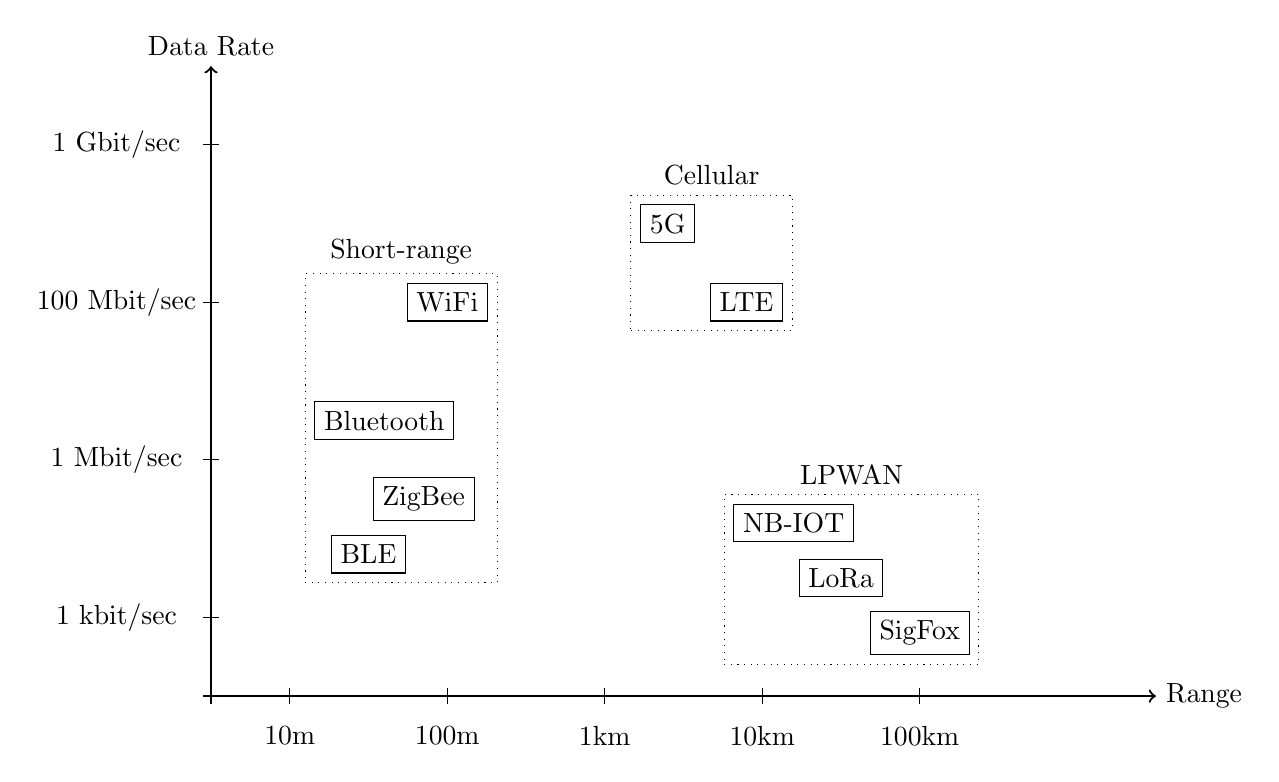
\begin{tikzpicture}
    \draw[->,thick] (-0.1,0)--(12,0) node[right]{Range};
    \draw[->,thick] (0,-0.1)--(0,8) node[above]{Data Rate};
    \node[] at (1, -0.5) {10m};
    \draw[] (1,-0.1)--(1,0.1);
    \node[] at (3, -0.5) {100m};
    \draw[] (3,-0.1)--(3,0.1);
    \node[] at (5, -0.5) {1km};
    \draw[] (5,-0.1)--(5,0.1);
    \node[] at (7, -0.5) {10km};
    \draw[] (7,-0.1)--(7,0.1);
    \node[] at (9, -0.5) {100km};
    \draw[] (9,-0.1)--(9,0.1);

    \node[] at (-1.2, 1) {1 kbit/sec};
    \draw[] (-0.1,1)--(0.1,1);
    \node[] at (-1.2, 3) {1 Mbit/sec};
    \draw[] (-0.1,3)--(0.1,3);
    \node[] at (-1.2, 5) {100 Mbit/sec};
    \draw[] (-0.1,5)--(0.1,5);
    \node[] at (-1.2, 7) {1 Gbit/sec};
    \draw[] (-0.1,7)--(0.1,7);
    
    \node[draw] at (8,1.5) (lora) {LoRa};
    \node[draw] at (9.0,0.8) (sigfox) {SigFox};
    \node[draw] at (7.4,2.2) (nb) {NB-IOT};
    \node[draw,dotted,fit=(lora) (sigfox) (nb), label=above:{LPWAN}] {};

    
    \node[draw] at (2.2,3.5) (bluetooth) {Bluetooth};
    \node[draw] at (2.7,2.5) (zigbee) {ZigBee};
    \node[draw] at (2.0,1.8) (ble) {BLE};
    \node[draw] at (3,5) (wifi) {WiFi};
    \node[draw,dotted,fit=(bluetooth) (zigbee) (ble) (wifi), label=above:{Short-range}] {};

    \node[draw] at (6.8,5) (lte) {LTE};
    \node[draw] at (5.8,6) (5g) {5G};
    \node[draw,dotted,fit=(lte) (5g), label=above:{Cellular}] {};
\end{tikzpicture}
\caption{Comparison of the existing IoT wireless technologies by range and data rate}
\label{fig:commrangegraph}
\end{figure}


This work focus only on \emph{LoRa}, a proprietary chirp spread spectrum modulation technique owned by \emph{Semtech} operating in the sub-GHz unlicensed \emph{ISM} band, that will be explained in more details in section \ref{section:lora}.
The main characteristics of \emph{LoRa} is that it trade throughput for range and low power transmission that as already achieved a record distance of 700km with direct line of sight between the receiver and the transmitter\footnote{https://www.thethingsnetwork.org/article/ground-breaking-world-record-lorawan-packet-received-at-702-km-436-miles-distance}. However this case is not a real world example, we should expect a typical range in urban areas of around \emph{~2-5km} and \emph{15km} in suburban areas\cite{8030482}. Fine tuning the \emph{PHY} settings of the protocol also allow to trade communication distance over throughput and a longer band usage which decrease the number of concurrent motes that can communicate over the band\cite{10.1145/2988287.2989163}.

\emph{LoRa} is often used in conjunction with the \emph{LoRaWAN} a point-to-multipoint protocols. \emph{LoRaWAN} is a ALOHA based\cite{loraalliance:lorawanspecification} network using a star-of-stars topology composed of
wirelessly interconnected \emph{motes} sending data to \emph{gateways} which relay messages to central servers over a Cellular or Ethernet connection as we can see in Figure \ref{fig:startopology}.

\begin{figure}[H]
\begin{subfigure}[b]{.5\textwidth}
    \centering
    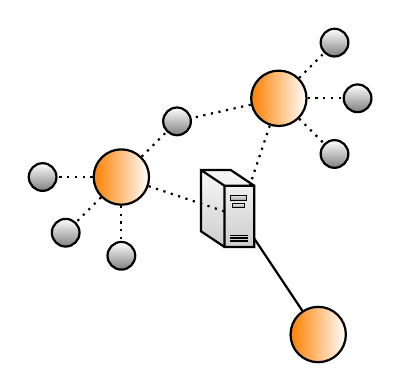
\begin{tikzpicture}[auto, thick]
      % Place super peers and connect them
      \foreach \place/\name in {{(0,-1)/a}, {(2,0)/b}, {(2.5, -3)/c}}
        \node[gateways] (\name) at \place {};
      \node[server] (d) at (1.5,-1.5) {};
      %
      \foreach \source/\dest in {a/d, b/d}
        \path[dotted] (\source) edge (\dest);
      \path (c) edge (d); % Non dotted
      %
      % Place normal peers
      \foreach \pos/\i in {above right of/1, right of/2, below right of/3}
        \node[motes, \pos =b ] (b\i) {};
      \foreach \speer/\peer in {b/b1,b/b2,b/b3}
        \path[dotted] (\speer) edge (\peer);
      %
      \foreach \pos/\i in {below left of/1, below of/2, left of/3, above right of/4}
        \node[motes, \pos =a ] (a\i) {};
      \foreach \speer/\peer in {a/a1,a/a2,a/a3,a/a4}
        \path[dotted] (\speer) edge (\peer);
      %
      \path[dotted] (b) edge (a4);
    \end{tikzpicture}
    \caption{Star topology}
    \label{fig:startopology}
\end{subfigure}
\hfill
\begin{subfigure}[b]{.5\textwidth}
    \centering
    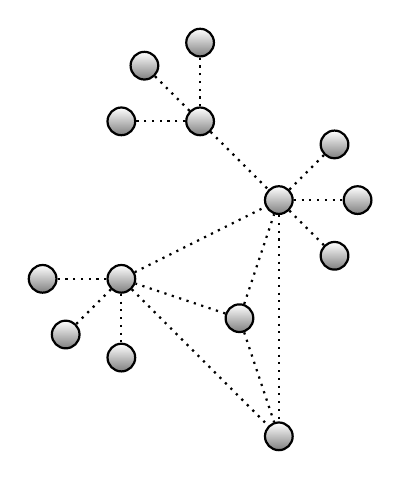
\begin{tikzpicture}[auto, thick]
      % Place super peers and connect them
      \foreach \place/\name in {{(0,-1)/a}, {(2,0)/b}, {(2, -3)/c}, {(1,1)/d}, {(1.5, -1.5)/f}}
        \node[motes] (\name) at \place {};
      \foreach \source/\dest in {a/b, a/c, b/c, d/b, f/a, f/b, f/c}
        \path[dotted] (\source) edge (\dest);
      %
      % Place normal peers
      \foreach \pos/\i in {above right of/1, right of/2, below right of/3}
        \node[motes, \pos =b ] (b\i) {};
      \foreach \speer/\peer in {b/b1,b/b2,b/b3}
        \path[dotted] (\speer) edge (\peer);
      %
      \foreach \pos/\i in {above left of/1, left of/2, above of/3}
        \node[motes, \pos =d ] (d\i) {};
      \foreach \speer/\peer in {d/d1,d/d2,d/d3}
        \path[dotted] (\speer) edge (\peer);
      %
      \foreach \pos/\i in {below left of/1, below of/2, left of/3}
        \node[motes, \pos =a ] (a\i) {};
      \foreach \speer/\peer in {a/a1,a/a2,a/a3}
        \path[dotted] (\speer) edge (\peer);
    \end{tikzpicture}
    \caption{Mesh Network Topology}
    \label{fig:meshtopology}
\end{subfigure}
\caption{Different LoRa Network Topologies}
\label{fig:topologies}
\end{figure}




The issue we have is \emph{LoRaWAN} does not scale\cite{10.1145/2988287.2989163}, especially in an urban environment where a lot of motes could overlap. \emph{LoRaWAN} is \emph{ALOHA} based and\emph{CSMA} is not possible because \emph{Channel Activity Detection} only detect the preamble of a communication. This mean a lot of collision can occur during a transmission attempt with a gateway. The \emph{LoRaWAN} protocol state that on collision occur the transmission has to be re-done which lead to a bigger energy consumption as well as occupying the channel even more.
Link quality may also vary some motes far away from the gateway may have issue with doing a correct transmission. Environmental factor like temperature, humidity\cite{evaluation_of_the_reliability_of_lora}, have a lot of influence in the link quality.

Also gateways may not be available everywhere, some use cases may not allow the the installation of gateways, which would imply a power and internet connection, that's the case for pipelines and tunnel, % cite here TODO
where we would prefer to only run devices on batteries.

\begin{figure}[H]
    \centering
    \def\angle{0}
    \def\radius{3}
    \begin{tikzpicture}[nodes = {font=\sffamily}]
      \foreach \color in {
            yellow,
            red,
            yellow,
            white,
            red,
            yellow,
            white,
            yellow,
            white,
            white,
            red,
            red,
        } {
        \ifx\color\empty\else
            \draw[fill={\color!50},draw={\color}] (0,0) -- (\angle:\radius)
              arc (\angle:\angle+30:\radius) -- cycle;
            \pgfmathparse{\angle+30}
            \xdef\angle{\pgfmathresult}
        \fi
        };
        \xdef\radius{2.5}
        \foreach \color in {
            yellow,
            red,
            yellow,
            yellow,
            red,
            white,
            yellow,
            red,
            white,
            white,
            white,
            white,
        } {
        \ifx\color\empty\else
            \draw[fill={\color!50},draw={\color}] (0,0) -- (\angle:\radius)
              arc (\angle:\angle+30:\radius) -- cycle;
            \pgfmathparse{\angle+30}
            \xdef\angle{\pgfmathresult}
        \fi
        };
        \xdef\radius{2}
        \foreach \color in {
            yellow,
            red,
            green,
            red,
            yellow,
            white,
            yellow,
            white,
            white,
            white,
            white,
            white,
        } {
        \ifx\color\empty\else
            \draw[fill={\color!50},draw={\color}] (0,0) -- (\angle:\radius)
              arc (\angle:\angle+30:\radius) -- cycle;
            \pgfmathparse{\angle+30}
            \xdef\angle{\pgfmathresult}
        \fi
        };
        \xdef\radius{1.5}
        \foreach \color in {
            yellow,
            red,
            yellow,
            yellow,
            yellow,
            green,
            yellow,
            white,
            red,
            white,
            white,
            white,
        } {
        \ifx\color\empty\else
            \draw[fill={\color!50},draw={\color}] (0,0) -- (\angle:\radius)
              arc (\angle:\angle+30:\radius) -- cycle;
            \pgfmathparse{\angle+30}
            \xdef\angle{\pgfmathresult}
        \fi
        };
        \xdef\radius{1}
        \foreach \color in {
            green,
            green,
            green,
            yellow,
            yellow,
            yellow,
            white,
            white,
            yellow,
            red,
            yellow,
            red,
        } {
        \ifx\color\empty\else
            \draw[fill={\color!50},draw={\color}] (0,0) -- (\angle:\radius)
              arc (\angle:\angle+30:\radius) -- cycle;
            \pgfmathparse{\angle+30}
            \xdef\angle{\pgfmathresult}
        \fi
        };
        \xdef\radius{0.5}
        \foreach \color in {
            green,
            green,
            yellow,
            yellow,
            green,
            green,
            yellow,
            red,
            yellow,
            green,
            green,
            green,
        } {
        \ifx\color\empty\else
            \draw[fill={\color!50},draw={\color}] (0,0) -- (\angle:\radius)
              arc (\angle:\angle+30:\radius) -- cycle;
            \pgfmathparse{\angle+30}
            \xdef\angle{\pgfmathresult}
        \fi
        };
    \end{tikzpicture}
\caption{Typical gateway coverage\cite{lorajambalaya}}
\label{fig:coverage}

\begin{tabular}{r@{: }l r@{: }l}

\begin{tikzpicture}\draw[fill=green,line width=1pt]  circle(1ex);\end{tikzpicture} & Good\ Connection & 
\begin{tikzpicture}\draw[fill=yellow,line width=1pt]  circle(1ex);\end{tikzpicture} & Intermediate\ Connection\\

\begin{tikzpicture}\draw[fill=red,line width=1pt]  circle(1ex);\end{tikzpicture} & Bad\ Connection & 
\begin{tikzpicture}\draw[fill=white,line width=1pt]  circle(1ex);\end{tikzpicture} & No\ Connection 
\end{tabular}
\end{figure}




% \begin{tikzpicture}
%     \node[draw] (Application) [abstract, rectangle]{\textbf{Application Layer}};
%     \node[draw] (MAC) [abstract, rectangle, below=0.2cm of Application, text justified]{\textbf{Media Access Control (MAC) Layer}};
%     \node[draw] (Phy) [abstract, rectangle, below=0.2cm of MAC, text justified]{\textbf{Physical (PHY) Layer}};
%     \node[draw] (Rf) [abstract, rectangle, below=0.2cm of Phy, text justified]{\textbf{Radio Frequency (RF) Layer}};
% \end{tikzpicture}

\paragraph{}

That why opting for a multi-hop solution instead of the star network has been proposed and can be an actual good idea to increase the redundancy and the reliability of the lossy network. Gateways are also sensible to power outage and can be a single point a failure of the network while a multi-hop network can adapt to this kind of topological changes. % TODO cite study with the roover water

One of the solution that arised from \emph{IoT} solutions is to use
Time-Slotted Channel Hopping communication to route.




\chapter{Context}

% As of today very little work has been done on creating a multihop LoRa Network (see Kris Paper on RPL LoRa in context section)

\section{LoRa}

\label{section:lora}

\paragraph{Packet Format}
\paragraph{Chirp Spread Spectrum (CSS) modulation}
\paragraph{Transmission Power}
\paragraph{Spreading Factor}

The higher the \emph{SF} the longer the communication range get while the transmission also get slower. Frames can be send at the same time if they are all sent with a different spreading factors\cite{8030482}.

The data rate can range from 0.3kbps to 27kbps depending on the \emph{SF} % TODO Calculation needed

\paragraph{Bandwidth}
\paragraph{Coding-Rate}
\paragraph{Channels}

% See 'Understanding the limits of LoRaWAN' the 3 channels definition in Europe

\paragraph{Time On Air}

\begin{equation}
  \label{eq:tsym}
  T_{sym} = \frac{2^{SF}}{BW}
\end{equation}
\begin{equation}
  \label{eq:tpreamble}
  T_{preamble} = (n_{preamble} + 4.25)T_{sym}
\end{equation}
\begin{equation}
  \label{eq:payloadsymnb}
  payloadSymbNb = 8 + \max(ceil(\frac{8PL - 4SF + 28 + 16 - 20H}{4(SF - 2DE)})(CR + 4),0)
\end{equation}
\begin{equation}
  \label{eq:tpayload}
  T_{payload} = payloadSymNb T_{sym}
\end{equation}
\begin{equation}
  \label{eq:tpacket}
  T_{packet} = T_{preamble} + T_{paylaod}
\end{equation}

\section{TSCH}

\section{6LoWPAN}

% 6TOP Sublayer

\section{Contiki OS}

\section{Related work}

\subsection{Time-Slotted LoRa}

\subsection{Multihop LoRa}

\chapter{Radio Driver for Zolertia with the RN2483 module\label{section:radio}}

% Most of the LoRaWAN features were not implemented or tested since this was out of the scope of this project.

The \emph{Zolertia RE-Mote REV-B} platform doesn't support \emph{LoRa} out of
the box. This chapter covers the implementation of a radio driver on
\emph{Contiki-NG} for the \emph{RN2483}, a LoRa module from Microhip,
communicating with the \emph{RE-Mote} platform.

\section{Preliminary work}

Last year \emph{Roald Van Glabbeek}, in the course of his master thesis~\cite{8847137}, 
aiming on doing further research on \emph{energy efficient lora multihop networks}, 
started working on the \emph{RN2483} module.
For this purpose he made \emph{RN2483 Shields} adapted to the pin
configuration of the \emph{Zolertia RE-Mote REV-B}. He also started a radio driver
implementation for Contiki-OS\@.

In a previous attempt to adapt \emph{TSCH} for \emph{LoRa}
in~\cite{njomgang_2018}, Serge did his experimentation with the \emph{LoRaMote}
demo platform from \emph{Semtech} using a different LoRa radio module the
\emph{SX1272}. 
As analyzed in~\cite{8847137}, LoRaMotes turned out to be an issue for the
further research because they were no longer produced, 
new versions were expensive and memory was a bottleneck.
That's why \emph{Zolertia RE-Mote} was chosen. The platform is already available 
and well maintained in \emph{contiki-ng} (making the transition faster and less
error prone as less code need to be developed) and the platform was already used 
in the \emph{ETRO Lab}.

The first part of my work consisted in implementing a reliable
and fully featured radio driver for the \emph{RN2483} module working in the last
version of \emph{contiki-ng}.

\section{RN2483 Module Structure}

Developed by \emph{Microchip} the \emph{RN2483} is a LoRa module operating in
the 433 MHz and 868 MHz Frequency Bands~\cite{microchip:rn2483}. 
The module is specifically designed to work with LoRaWAN compatible networks, 
by including a set of commands designed for seamless integration with the
\emph{LoRaWAN Protocol Stack}

All communication to and from the module are done via \emph{UART} ASCII command,
making it easy for a human to interact with the module by handwriting commands
on a terminal and reading the response back in a readable format
(see~\ref{fig:pconn}).
% The module is made for ease of use over performance and power consumption.

\begin{figure}[H] % TODO More info on axis
\centering
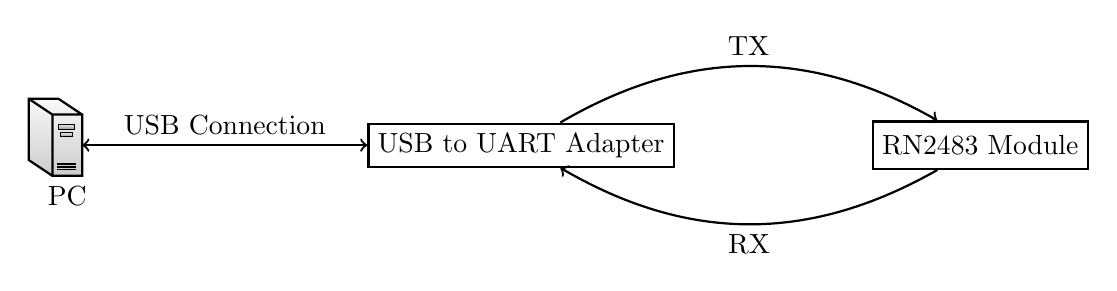
\begin{tikzpicture}[auto, thick]
  \node(pc) [server, label=below:{PC}] {};
  \node(ftdi) [draw, rectangle, right=of pc, right=4cm] {USB to UART Adapter};
  \node(module) [draw, rectangle, minimum size=6mm, right=of ftdi, right=2.5cm] (module) {RN2483 Module};

  \path (pc) edge[<->] node[]{USB Connection} (ftdi) ;
  \path (ftdi) edge[->,bend left] node[text width=1cm, align=center]{TX} (module);
  \path (module) edge[->,bend left] node[text width=1cm, align=center]{RX} (ftdi);
\end{tikzpicture}
\caption{Simple communication with the module scenario\label{fig:pcconn}}
\end{figure}


The module's interface include three types of commands that enable access to
different functions~\cite{microchip:reference}.

\begin{itemize}
  \item \emph{radio} for the low-level radio commands to access the transceiver
    and PHY settings directly without the LoRaWAN interface overhead.
  \item \emph{mac} to access the LoRaWAN protocol stack configurations and
    commands. This command set will be used less as our implementation require 
    low-level transceiver access.
  \item \emph{sys} for the module specific configurations such as the module
    GPIOs state, \emph{sleep}, EEPROM memory access, \ldots
\end{itemize}

\section{Testing Setup}

My testing setup was the same as~\cite{8847137}. I used a Zolertia RE-Mote
Rev-B platform, using the CC2538 microcontroller, connected to a
RN2483 breakout board, as schematized in Fig~\ref{fig:schemaconn}. 

The RE-Mote platform has two UART peripheral and we are using the UART1 peripheral 
to communicate with the module instead of UART0, already used by the platform USB 
debugger.

The reset pin of the module was wired to the \lstinline{PD0} GPIO to allow
software reset of the module as well as a push button for hard reset.

\begin{figure}[H]
  \centering
  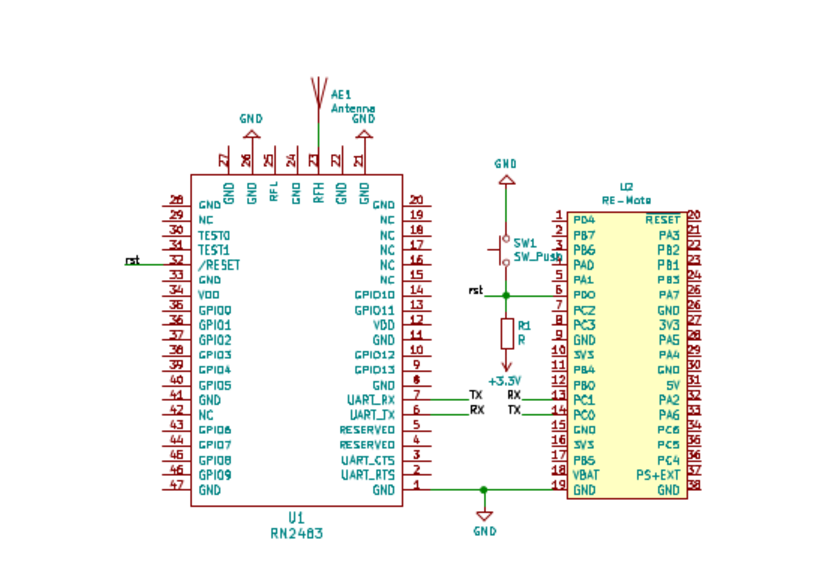
\includegraphics[scale=0.70]{thesis.tex/chapters/driver/fig/conn_diag.pdf}
  \caption{Hardware connection\label{fig:schemaconn}}
\end{figure}

\section{Implementation}

All the files for the driver implementation are available in
\lstinline{/arch/dev/rn2483} and examples are located in
\lstinline{/examples/platform-specific/rn2483}.

\subsection{Structure}

My implementation structure was inspired by the work in~\cite{8847137} as well
as the \emph{RIOT-OS} project\footnote{\url{https://github.com/RIOT-OS/RIOT}}, which
already took care to define a lot of the parameters we want to use with the
module.

Following, is a listing of the different files I created and their usage.

\begin{description}
  \item[lora] LoRa radio specific functions, declaration and configuration. This
    include functions used to calculate the time on air as well as
    LoRa PHY configuration structure and parameters.
  \item[rn2483-include] This file contain the declaration both needed by
    \lstinline{rn2483-uart} and \lstinline{rn2483} to avoid cycling inclusion
    that mess with the compiler.
  \item[rn2483-uart] Lower level implementation of the function to directly
    communicate with the module via UART\@. This part is the closest one to the
    hardware because of the uart implementation being specific to the CC2538.
  \item[rn2483-api] Complete coverage of the RN2483 commands. Using functions
    from this file allow the user of the driver to not bother writing
    each command by hand and use a standardized structure instead.
  \item[rn2483] Implementation of the Contiki radio device driver. The file
    contain the standardized way of Contiki to use and configure a radio device.
    This is the structure shared by all the radio driver in Contiki.
\end{description}

\subsection{Synchronous communication with the module}

The first design challenge of the driver implementation is to create a
synchronous mechanism to receive message from the UART\@. 
The need for synchronous messaging is crucial since every
transmission, configuration and reception are done via UART\@.
Acknowledgements from commands are mandatory to avoid command
clash when trying to use the module at the same time.
The previous implementation in~\cite{8847137} used fixed time delays to 
wait for the command to be fully executed on the module. However, this method 
quickly showed its own limitation, each commands has their own delays and a
fixed delay slow down the global execution.

% TODO Maybe sequence diagram with a clash

The UART driver implementation for the CC2538 in Contiki don't have a synchronous 
blocking read function out of the box, it assume the programmer will compute the
responses from UART in processes instead by waiting for event instead.
The way the reception is working is by executing a so called \emph{input handler} 
at each interruption triggered by UART reception.
The default input handler is the \lstinline{serial_line_input_byte} 
specifically designed for serial communication with a terminal and we will keep
using this handler with UART0 to get debug messages with a USB connection from 
a computer.

However, we have to define our own handler for the UART1 peripheral directly
connected with the module.
It will be similar as the default one because they are both using same message
structure terminating by \lstinline{\r\n}, but 
where \lstinline{serial_line_input_byte} is passing each character to a standalone
process (called \lstinline{serial_line_process}) broadcasting an event when the 
command is fully received, our handler is directly threating the message in the 
interrupt.

Working with processes and events, is not possible in our use case because Contiki 
don't have any mechanisms allowing programmers to wait for an event inside a 
function. Instead, Contiki allow to only wait for specific events inside
processes, but doing everything inside a big process is not an option.
The custom handler is designed as a state machine (Fig~\ref{fig:cmdstate}) and 
work with its own reception buffer. It takes advantage of the limited response 
format from the RN2483 module to sort each new communications.

\begin{itemize}
  \item Messages starting with \lstinline{radio rx  } are asynchronous LoRa
    radio messages.
  \item \lstinline{radio_tx_ok} indicate the end of a radio transmission. This
    implies we have done a transmission before.
  \item \lstinline{ok} indicate the acknowledgement of a command.
\end{itemize}

% Talk about the state machine

I implemented helper functions, to ease the command transmission and
acknowledgement between the RE-Mote and the RN2483.

\begin{description}
  \item[rn2483\_receive\_synch] busywait on the command states
    (Fig~\ref{fig:cmdstate}) until the \emph{received} state is 
    reached, or after the timeout has elapsed.
  \item[rn2483\_send\_cmd] a \emph{printf} style command, automatically 
    waiting for acknowledgement (with the possibility to add a custom timeout).
  \item[rn2483\_raw\_cmd] sending the command from a buffer in argument
    without formatting or waiting for acknowledgement.
\end{description}

\begin{figure}[H]
\centering
  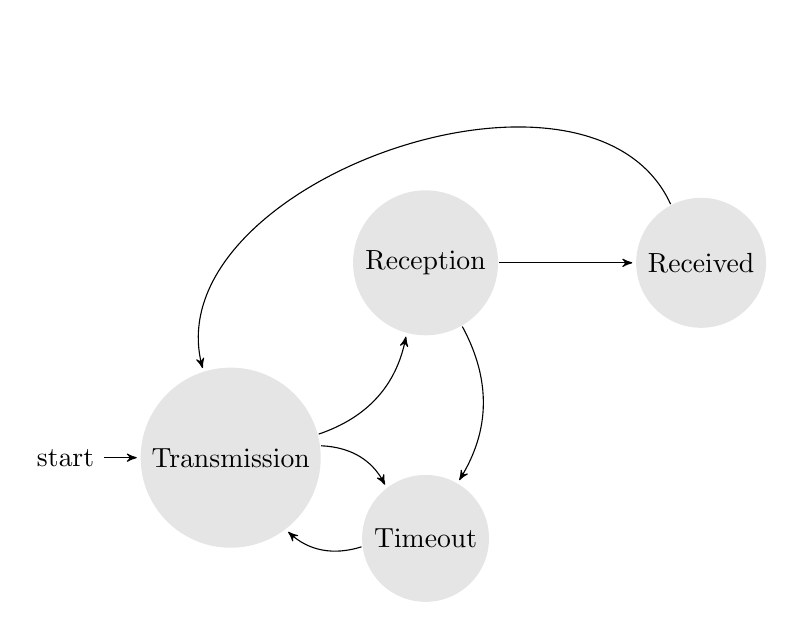
\begin{tikzpicture}[->,>=stealth',shorten >=1pt,auto,node distance=3.5cm]
  \tikzstyle{every state}=[thick,draw=gray!50,fill=gray!20,draw=none,text=black]

  \node[initial,state] (A)                    {Transmission};
  \node[state]         (B) [above right of=A] {Reception};
  \node[state]         (C) [below of=B]       {Timeout};
  \node[state]         (D) [right of=B]       {Received};

  \path (A) edge [bend right]    node {     } (B)
            edge [bend left]     node {     } (C)
        (B) edge [bend left]     node {     } (C)
            edge                 node {     } (D)
        (C) edge [bend left]     node {     } (A)
        (D) edge [bend right=85] node {     } (A);
\end{tikzpicture}
\caption{The command states\label{fig:cmdstate}}
\end{figure}


\subsection{Transmission}

The radio transmission command has a different pattern from the other commands 
of the module. After the acknowledgement of the radio transmission 
command (\lstinline{radio tx ...}) the module will also send a second message
when the message is fully transmitted.

\begin{figure}[H]
\centering

\begin{sequencediagram}

\newthread{A}{RE-Mote}{}
\newinst[1]{B}{RN2483}{}
\newinst[3]{C}{Radio Band}{}
\begin{call}{A}{radio tx~\ldots}{B}{radio\_tx\_ok}
  \messdash{B}{ok}{A}
  
  \begin{sdblock}{Radio Transmission}{Transmition time calculated
    in~\ref{eq:tpacket}}
    \begin{call}[4]{B}{}{C}{}
    \end{call}
  \end{sdblock}
\end{call}

\end{sequencediagram}

  \caption{\lstinline{radio tx} command sequence diagram\label{fig:txsequence}}

\end{figure}



Microchip chose to represent the payload as string formatted hex number to
facilitate the manual writing of commands, making the message payload twice as
long as its original content. As all the content we will handle 
are represented as \emph{8 bit} number array, a function to convert array to
string representation and vice versa was taken from the RIOT-OS project.

\subsection{Asynchronous Reception}

The last component of a complete driver implementation is to receive radio
messages.
Reception follow a different scheme from the other commands, a message
reception can happen at any time asynchronously from the moment we run the
command \lstinline{radio rx 0}.
To tackle this issue a one message inbox has been implemented (see
Fig~\ref{fig:rxstate}).
At the reception of a command from the module we look at the structure of
the message.
Every message coming from a radio communication start with \lstinline{radio rx  }, 
if it follow this structure a flag is set and is unset at the moment we read the
message from our code.
Messages are received in a string formatted hex number, we must convert it to an
\emph{8 bit integer array}. 
% TODO Talk about packet buf ?
% We don't store the final result in the same buffer as the one used for
% reception as reading the result 
% This array is stored in a different place than the received message as command
% may be executed between the moment we receive the message and the moment we
% read it.
Also, a timestamp is saved at the reception to keep track of when was received the
message.

\begin{figure}[H]
\centering
  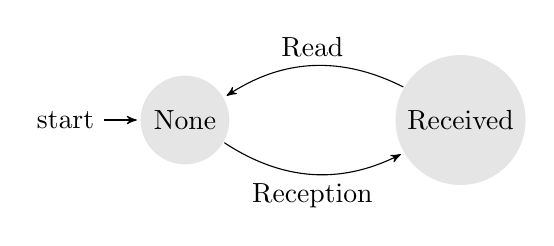
\begin{tikzpicture}[->,>=stealth',shorten >=1pt,auto,node distance=3.5cm]
  \tikzstyle{every state}=[thick,draw=gray!50,fill=gray!20,draw=none,text=black]

  \node[initial,state] (A)              {None};
  \node[state]         (B) [right of=A] {Received};

    \path (A) edge [bend right] node[below] {Reception} (B)
          (B) edge [bend right] node[above] {Read} (A);
\end{tikzpicture}
\caption{The RX states\label{fig:rxstate}}
\end{figure}


\subsection{Contiki Radio Driver}

The Contiki wiki didn't provided any information about writing our own radio driver
or porting a new radio platform for Contiki.
I based my implementation on the other radio driver implementation already
available on Contiki to understand the driver structure.

To create a Contiki radio driver we have to implement a \lstinline{radio_driver}
structure that must implement the following functions.

\begin{description}
  \item[init] is the first function of the driver executed at startup.
    This is where the configuration of the RN2483 take place
    as well as setting the module into point-to-point mode to not use the default
    LoRaWAN stack.
  \item[prepare] is the function called before a transmission with the data we
    want to transmit as parameter. 
    We can't transmit radio messages while listening for incoming messages, the
    first step of preparation is to exit the radio reception mode with the
    command \lstinline{radio rxstop}.
    The command also take care to convert the data to the hex string and
    already format the radio command ready to be sent.
  \item[transmit] send the already formatted command in the prepare function and
    wait for the \lstinline{radio_tx_ok} acknowledgement.
  \item[send] is the combination of prepare and transmit.
  \item[read], when a new message is received in the inbox, copy the radio
    message to the buffer passed in argument.
  \item[channel\_clear]
  \item[receiving\_packet] should theoretically check if the radio module is
    currently getting a new message from a transmission. This is a function we
    can expect from some platform with integrated radio module but here the
    simplicity of the RN2483 show his limit and I found no way for the module
    to acknowledge when it's receiving a new message.
  \item[pending\_packet] check the message inbox to see if we received a new
    message.
  \item[on] wake-up the module and start listening to radio messages.
  \item[off] stop listening to radio messages and put the module to sleep.
  \item[get\_value, set\_value, get\_object, set\_object] are all function used
    to configure the radio driver in a streamlined way. The parameter we need to
    implement will be discussed in Chapter~\ref{section:tsch}.
\end{description}

% TODO talk about Poll mode

\section{Validation test}

% Talk about project configuration like with the NETSTACK

To verify the implementation of the radio driver two examples were made.

\begin{itemize}
  \item The \emph{RN2483 shell} available in
    \lstinline{/example/platform-specific/lora/rn2483} is a tool to interact
    directly with the module.
  \item The \emph{ping-pong} example based on the nullnet example already
    available in \emph{contiki-ng} located in 
    \lstinline{/example/platform-specific/lora/nullnet} demonstrate the driver
    is correctly working with upper layer of the network stack.
\end{itemize}

For each Contiki project, the different OSI layers are defined using the
\emph{Contiki's Network Protocol stack}, or \lstinline{NETSTACK}, to select
each layer specific implementation we want to use in our project (Fig~\ref{fig:netstack}).
Also, each project are usually bundled with a \lstinline{project-conf.h}
configuration file where we can define the parameter of our project. 
To set my LoRa driver as the physical layer implementation we must add this line to
each \lstinline{project-conf.h}.

\begin{lstlisting}
#define NETSTACK_CONF_RADIO                        rn2483_radio_driver
\end{lstlisting}

\begin{figure}[H]
\centering
  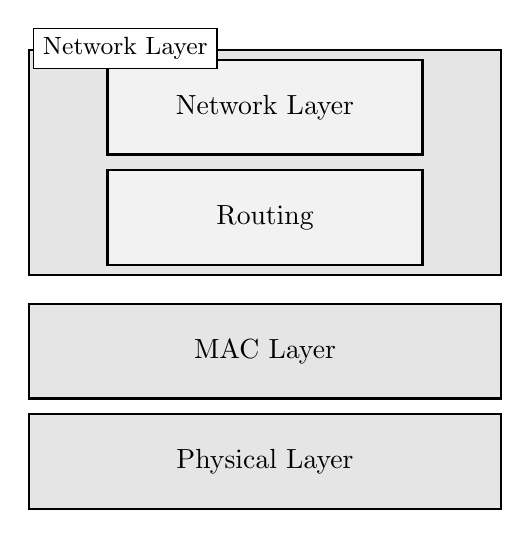
\begin{tikzpicture}[->,>=stealth',shorten >=1pt,auto,node distance=1.4cm]

  \tikzstyle{comment}=[
    right=2pt,
    font=\small,
    fill=white,
    text=black,
    draw=black,
  ]

  \tikzstyle{every state}=[rectangle,thick,
    draw=black,fill=gray!20,text=black,
    minimum width= 6cm,
    minimum height= 1.20cm
  ]

  \tikzstyle{smallstate}=[rectangle,thick,
    draw=black,fill=gray!10,text=black,
    minimum width= 4cm,
    minimum height= 1.20cm
  ]

  \node[smallstate]         (A)                    {Network Layer};
  \node[smallstate]         (B) [below of=A]       {Routing};
\begin{scope}[on background layer]
  \node[state, fit=(A)(B)] (AB)                 {};
\end{scope}
  \node[state,below=1cm]         (C) [below of=AB]       {MAC Layer};
  \node[state]         (D) [below of=C]       {Physical Layer};

  \node[comment]       at (AB.north west) {Network Layer};
  % \node[comment]       at (C.north west) {MAC Layer};
  % \node[comment]       at (D.north west) {Physical Layer};
  % \path (A) edge [bend right]    node {     } (B)
  %           edge [bend left]     node {     } (C)
  %       (B) edge [bend left]     node {     } (C)
  %           edge                 node {     } (D)
  %       (C) edge [bend left]     node {     } (A)
  %       (D) edge [bend right=85] node {     } (A);
\end{tikzpicture}
\caption{The Contiki's Network Protocol Stack\label{fig:netstack}}
\end{figure}


\subsection{Shell}

This example extend the existing shell available in Contiki by writing a set
of commands to test and interact with the the RN2483 via UART\@.

Here is the list of the added commands to the Contiki shell.

\begin{lstlisting}
'> sys': Send a 'system' command to the RN2483 Module.
'> mac': Send a 'mac' command to the RN2483 Module.
'> radio': Send a 'radio' command to the RN2483 Module.
'> tx': Transmit a radio message with the RN2483.
'> sleep': Put RN2483 into sleep mode.
'> wakeup': Force wakeup of RN2483.
'> rn2483_reset': Hardware Reset of the RN2483 Module.
'> help': Shows this help.
\end{lstlisting}

This was used during the development of the driver as a way to test parameters
as well as the synchronous communication implementation.

\subsection{Ping-Pong}

I based this example on the \emph{nullnet-broadcast} example to test if two
node could communicate using the LoRa driver I implemented when controlled by
the \emph{CSMA} MAC layer instead of directly using the driver API\@.

The example is using the NETSTACK in Fig~\ref{fig:pingpongstack}.

\begin{figure}[H]
\centering
  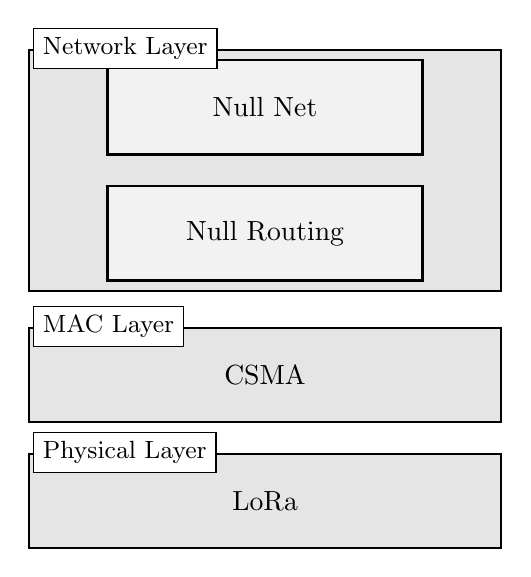
\begin{tikzpicture}[->,>=stealth',shorten >=1pt,auto,node distance=1.6cm]

  \tikzstyle{comment}=[
    right=2pt,
    font=\small,
    fill=white,
    text=black,
    draw=black,
  ]

  \tikzstyle{every state}=[rectangle,thick,
    draw=black,fill=gray!20,text=black,
    minimum width= 6cm,
    minimum height= 1.20cm
  ]

  \tikzstyle{smallstate}=[rectangle,thick,
    draw=black,fill=gray!10,text=black,
    minimum width= 4cm,
    minimum height= 1.20cm
  ]

  \node[smallstate]         (A)                    {Null Net};
  \node[smallstate]         (B) [below of=A]       {Null Routing};
\begin{scope}[on background layer]
  \node[state, fit=(A)(B)] (AB)                 {};
\end{scope}
  \node[state,below=1cm]         (C) [below of=AB]       {CSMA};
  \node[state]         (D) [below of=C]       {LoRa};

  \node[comment]       at (AB.north west) {Network Layer};
  \node[comment]       at (C.north west) {MAC Layer};
  \node[comment]       at (D.north west) {Physical Layer};
  % \path (A) edge [bend right]    node {     } (B)
  %           edge [bend left]     node {     } (C)
  %       (B) edge [bend left]     node {     } (C)
  %           edge                 node {     } (D)
  %       (C) edge [bend left]     node {     } (A)
  %       (D) edge [bend right=85] node {     } (A);
\end{tikzpicture}
\caption{The network stack used for the ping-pong example\label{fig:pingpongstack}}
\end{figure}


The example is a simple two-way communication between two RE-Motes. 
The first one is sending a request with a number as
payload and wait for the acknowledgement from the second motes sending back
the same payload. 
No other request is sent until the acknowledgement is received.
This is schematized in Fig~\ref{fig:pingpongsequence}.

The two different implementation to setup on each nodes are available in the
example folder.

\begin{itemize}
  \item \lstinline{ping.c} send the request and wait for acknowledgement.
  \item \lstinline{pong.c} send the acknowledgement.
\end{itemize}

\begin{figure}[H]
\centering

\begin{sequencediagram}

\newthread{A}{Mote A}{}
\newinst[1]{B}{Mote B}{}

\begin{call}[4]{A}{ping}{B}{pong}
\end{call}
\end{sequencediagram}

\caption{Description of the execution of the ping-pong example\label{fig:pingpongsequence}}

\end{figure}




\chapter{Time-Slotted Channel Hopping Implementation for LoRa\label{section:tsch}}

\section{Porting TSCH}

\subsection{Channels}

\subsection{Timestamp}

\subsection{Radio delay}

\subsection{$\mu s$ and rtimer ticks conversion}

\subsection{LoRa Time On Air}

\section{Adaptation of the timing}

\paragraph{Timing size issue}

\section{Testing}

\section{Considerations}


\chapter{Conclusion and further work}

\newpage

\printbibliography

\newpage

\section{Appendix}

\end{document}

